% !TEX root =  ./main.tex

\section{Introduction}

We explore the capabilities of a state-of-the-art toolset based on graph transformation to perform reachability, causal analysis and verification of complex systems modelled using Reaction Systems.

Reaction systems (RSs)~\cite{DBLP:journals/fuin/EhrenfeuchtR07} are a computational model inspired by the functioning of biochemical reactions within living cells. 
%The primary motivation behind RS is to provide a simple yet expressive model for understanding and analysing processes in natural and artificial systems.
RSs focus on the interaction of entities through a set of reactions. 
Each reaction relies on some reactants, inhibitors, and products to mimic two fundamental mechanisms found in nature: facilitation and inhibition.
%Facilitation means that a reaction can occur only if all of its reactants are present, while inhibition means that a reaction cannot occur if any of its inhibitors is present. 
At each time instant, the next state of the system is determined by the products of all enabled reactions plus some additional entities that are possibly provided by the environment.
Unlike traditional models of concurrency, like Petri nets, the theory of RSs is based on three principles: \emph{no permanency}: any entity vanishes unless it is sustained by a reaction; \emph{no competition}: an entity is either available for all reactions, or it is not available at all; and \emph{no counting}: the exact concentration level of available entities is ignored.
Moreover, due to the use of inhibitors, RS can exhibit non-monotonic behaviour, in the sense that what can be done with fewer resources is not necessarily replicable with more resources.

While \emph{closed} RSs evolve in isolation, \emph{interactive processes} are dealt with by providing suitable environments that provide a sequence of stimuli at each step: these are sets of entities that can be used to trigger or inhibit some reactions. A common example involves using contexts to analyse how drug administration affects organisms that are modelled as sets of reactions.

Since their introduction, RSs have been successfully applied to the analysis of complex systems in many different fields~\cite{ABP14,CMMBM12,Az17,OY16,DBLP:journals/ijfcs/EhrenfeuchtMR10,DBLP:journals/ijfcs/EhrenfeuchtMR11}.
Recent applications concerned, e.g., with the efficacy of medical treatments for comorbidities and with the selection of the best environment to achieve some desired phenomena~\cite{DBLP:conf/cmsb/BowlesBBFGM24,datamod2023}, led to experimenting with environments that exhibit nondeterministic and recursive behaviour.
As a consequence, performing reachability and causal analysis requires the exploration of large state spaces, for which the prototype tool \BioResolve~\cite{DBLP:journals/tcs/BrodoBF21} struggled in terms of  memory consumption and response time.
 
Graph Transformation (GT)~\cite{DBLP:series/eatcs/EhrigEPT06,DBLP:books/sp/HeckelT20} is a modelling technique that is widely applicable in problem domains where the objects of study have an inherent graphical structure, and the task at hand is to study their properties and evolution. Besides the graphs themselves, the core concept is that of a (transformation) \emph{rule} capturing a particular change to such a graph. Rules can be used, for instance, to describe the change of a system over time, but can also be instrumental in composing and decomposing graphs and so exposing structural properties.
Since RSs can be derived from Boolean network models and visualised themselves as suitable networks of reactions, it is quite natural trying to embed them within the GT framework to take advantage of well established analysis techniques.\footnote{\textcolor{blue}{It should be noted that there is another, quite unrelated, way in which the concepts of Graph Transformation and Reaction systems may be combined, namely by extending the latter from pure entities (which are analogous to graph nodes) to entities with relations between them (which can be encoded through graph edges). In \cite{DBLP:journals/jlap/KreowskiR19} this has inspired a new methodology for Graph Transformation, there called \emph{graph surfing}.}}

Importantly, from a practical point of view, there are a number of (academic) tools supporting the use of GT. The research described here crucially relies on \href{https://groove.cs.utwente.nl}{\GROOVE}~\cite{DBLP:journals/sttt/GhamarianMRZZ12}, one of the most prominent tools in this area, which was designed precisely to enable GT-based system analysis of the kind described above. The features of \GROOVE that are essential for the purpose of this research are:
\begin{enumerate}%[label=\emph{(\roman*)}]
\item Nested (i.e., quantified) rules, which capture simultaneous changes in all neighbourhoods that satisfy certain application conditions, rather than only locally in one such neighbourhood at a time; 
\item Complete exploration of the set of reachable states (under the given rules) using various strategies;
\item Model checking functionalities that can be used to validate previous findings as well to explore and support the study of new behavioural and structural properties.
\end{enumerate}

The main research question that motivated our study is: 
\emph{how can GT help in addressing the analysis of Reaction Systems?} 
To this aim, we encode a given RS as a single graph, upon which a small number of (fixed) rules can simulate the correct semantics. 

\begin{figure}
\centering
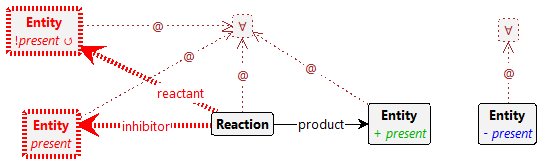
\includegraphics[scale=.42]{react}
\caption{Rule for reactions firing}
\label{fig:reactionfiring}
\end{figure}

The core rule describes the simultaneous firing of all \blab{Reaction}s of which no \lab{inhibitor}s and all \lab{reactant}s are present; the firing results in the presence of all \lab{product}s. Simultaneously, all currently present \blab{Entity}s are removed. In \GROOVE syntax, the core rule is drawn as in \Cref{fig:reactionfiring}.
To parse this, note that (in the \GROOVE notation) the red structure must be absent for the rule to apply; moreover, green labels are added and blue ones deleted upon rule application. The \ilab{present} flag signals whether an \blab{Entity} is considered to be currently present; hence, creating or deleting that flag comes down to creating or deleting the \blab{Entity}. The $\forall$-nodes impose the desired quantification, causing a single application of this rule to model the firing of all enabled \blab{Reaction}s, even if there are thousands of them.
Similarly for the simultaneous deletion of all \blab{Entity}s.

Our model also supports environments that inject \blab{Entity}s in a controlled manner. This is achieved by encoding the context specification in the initial graph and exploiting a second predefined rule, not shown here (see \Cref{fig:context}). A configuration is reachable if it can be constructed by the alternating application of both rules: first the context produces a set of stimuli (possibly upon inspection of the current state, but also nondeterministically or a combination of both), and then all enabled reactions are executed.

After a brief account of RSs (\Cref{sec:RS}) and \GROOVE (\Cref{sec:GTS}), we present the overall rationale, blueprint and key features of our approach in \Cref{sec:RS2GTS} through a simple vending machine example (\Cref{sec:student}).
The subsequent experimentation in \Cref{sec:experiments} is concerned with revisiting existing RS case studies to assess how \GROOVE can enhance their analysis. 
In particular, we tackle 
the comorbidity treatment scenario from~\cite{DBLP:conf/cmsb/BowlesBBFGM24} in \Cref{sec:cmsb2024}, 
the protein signalling networks analysis from~\cite{DBLP:conf/cmsb/BallisBFO24} in \Cref{sec:ccReact}, and
the T cell differentiation study from~\cite{datamod2023} in \Cref{sec:datamod2023}.
Our results are encouraging: \GROOVE is capable to explore large RSs 
%is well beyond what other tools have been able to achieve, 
by using roughly one tenth of the time compared to \BioResolve for both reachability and causal analyses.
More precisely, we are able to find a trace towards unwanted patterns (if they exist) among hundreds of thousands of reachable configurations using different heuristics; then, we can also prune the trace to extract a graphical representation of the causal history of that entities. Using the built-in model checker it is also possible to confirm the results of previous studies, as well as proving new facts.
A comparison with related tools is drawn in \Cref{sec:related}. Concluding remarks and future directions are discussed in \Cref{sec:conc}.
